\documentclass[a4paper,10pt]{article}

\usepackage[dutch]{babel}
\usepackage{graphicx}
\usepackage{amsmath}
\usepackage{amssymb}
\usepackage{amsthm}
\usepackage{wasysym}
\usepackage{float}
\usepackage{listings}
\usepackage{setspace}
\usepackage{tikz}
\usetikzlibrary{arrows}
\onehalfspacing

\DeclareGraphicsExtensions{.pdf,.png}

\begin{document}
\lstset{language=Haskell}
\title{Verslag 2: Lazy evaluation door middel van graafreductie}
\author{Koen Pauwels}
\maketitle

\section{Inleiding}
\subsection{Waarom lazy evaluation?}
\paragraph{}
In de meeste programmeertalen worden argumenten aan een functie ge{\"e}valueerd voordat de functie wordt opgeroepen.
Dit noemen we een \emph{call by value} strategie.
Het is echter mogelijk dat een argument nooit wordt gebruikt in de functie.
In dat geval wordt er overbodig werk geleverd.
\paragraph{}
We kunnen proberen dit overbodig werk te vermijden door de evaluatie van een argument uit te stellen totdat de waarde ervan nodig is.
Dit noemen we een \emph{call by need} of \emph{lazy evaluation} strategie.
Deze strategie is zo goed als uniek voor zuiver functionele talen.
In imperatieve talen berust de betekenis van een programma op het in een correcte, voorspelbare volgorde plaatsvinden van bepaalde \emph{side-effects}.
Met \emph{call by need} kan het erg moeilijk worden om uit te werken in welke volgorde de expressies zullen worden ge{\"e}valueerd, en dus in welke volgorde de side-effects zullen plaatsvinden.

\subsection{Waarom een graafvoorstelling?}
Wanneer een $\lambda$-expressie wordt ingeladen in de compiler, zal deze een boomvoorstelling van de expressie genereren.
Zoals eerder vermeld worden argumenten aan functies enkel ge{\"e}valueerd wanneer de waarde nodig is.
Na{\"i}eve normal-order reductie op de boomvoorstelling van de $\lambda$-expressie voldoet wel aan deze voorwaarde, maar zal vaak tot dubbel werk (en dus tot grote ineffici{\"e}nties) leiden.
Wanneer een parameter namelijk meerdere keren voorkomt in het lichaam van een expressie, zal elk voorval van die parameter vervangen moeten worden door een kopie van het argument.
Als we het programma voorstellen als een graaf in plaats van een boom, dan kunnen we elk voorval van de parameter in het lichaam van een $\lambda$-expressie vervangen door een \emph{referentie} naar het argument, in plaats van een kopie ervan.
Bij het evalueren van een argument zullen we ervoor zorgen dat de wortelnode van het argument wordt overschreven met het resultaat van de evaluatie.
Elke referentie naar het argument verwijst dan automatisch en zonder extra kost naar het resultaat van de evaluatie.

\subsection{Ori{\"e}ntatie in het project}
Het gehele project betreft een compiler die een zuiver functionele taal via verrijkte $\lambda$-calculus vertaalt naar gewone $\lambda$-calculus.
De bekomen $\lambda$-calculus expressie wordt dan gereduceerd in een \emph{runtime omgeving} die een graafreductiealgoritme toepast en de resultaten uitprint.
Dit verslag betreft deze runtime omgeving.

\section{Programmarepresentatie}
De graafvoorstelling moet alle constructies van de $\lambda$-calculus ondersteunen, maar verder verwachten we ook ondersteuning voor een aantal bijzondere builtin operaties en datastructuren.
In theorie is de $\lambda$-calculus voldoende om alle programma's die we wensen uit te drukken, maar in praktijk willen we onder meer de machinevoorstelling gebruiken voor getallen, machine-operaties kunnen uitvoeren op die getallen, gestructureerde datatypes kunnen gebruiken, etc.
\paragraph{}
De basis van de graafvoorstelling is de \emph{cel}, een eenvoudige datastructuur die uit drie elementen bestaat: een \emph{tag} die aangeeft over welk type cel het gaat, en twee \emph{fields}.
Een field kan een pointer naar een andere cel bevatten (op deze manier worden de edges van de graaf ge{\"i}mplementeerd), of een waarde waarvan de betekenis afhangt van het type cel en de context.

\begin{figure}[h]
    \begin{lstlisting}[language=C,frame=single,caption={Definitie van de Cell datastructuur}]
typedef enum {VAR, APP, ABSTR, DATA, BUILTIN, CONSTR} Tag;
union Field {
	struct Cell* ptr;
	char* sym;
	int num;
	Builtin op;
	StructuredDataTag data_tag;
	StructuredDataPtr data_ptr;
};
struct Cell {
	Tag tag;
	union Field f1;
	union Field f2;
};
\end{lstlisting}
\end{figure}

De eerste drie celtypes implementeren de structuren van de $\lambda$-calculus, zoals beschreven in \emph{The Implementation of Functional Programming Languages (IFPL)}: variabelen, applicaties en abstracties.
\begin{itemize}
\item
  Een \texttt{VAR} cel gebruikt slechts 1 van zijn fields.
  Dat veld bevat een pointer naar een string die het symbool opslaat.
  Er is een effici{\"e}ntere implementatie mogelijk: we zouden bij het compileren elk symbool kunnen associ{\"e}ren met een uniek getal, en dit getal rechtstreeks in het veld opslaan.
  Ik heb besloten om de originele namen te behouden om debugging niet te bemoeilijken.
\item
  De velden van een \texttt{APP} cel zijn eenvoudigweg celpointers naar de operator en de operand van een applicatie.
\item
  Een \texttt{ABSTR} cel bevat een pointer naar het parameter symbool, en een celpointer naar het lichaam van de functie.
\end{itemize}

Het boek is minder helder over welke extra tags er nodig zijn om de implementatie te vervolledigen.
Mijn implementatie maakt verder nog onderscheid tussen datacellen, builtins (operatoren en constanten) en constructors.
\begin{itemize}
\item
  \texttt{DATA} cellen worden gebruikt om gegevens in op te slaan.
  \emph{IFPL} lijkt onderscheid te maken tussen cellen die getallen opslaan en cellen die lijsten (\texttt{CONS} cellen) opslaan, en eventueel nog aparte structured data cellen.
  Ik zag geen reden om de data cellen bewust te maken van de betekenis van de gegevens die ze dragen, aangezien dit steeds af te leiden valt uit de context.
  Een functie die iets met de data doet, bevat genoeg informatie om de data te interpreteren.
  \texttt{DATA} cellen worden dus zowel gebruikt om primitieve data in op te slaan, zoals integers, of om naar gestructureerde datastructuren te verwijzen.
  In het eerste geval bevat de datacel enkel de waarde van de primitieve data.
  In het tweede geval bevat de cel een \emph{structured data tag} en een pointer naar de datastructuur.
  Wanneer de datastructuur werd aangemaakt door een constructor van een somtype, is het de structured data tag die onthoudt welke constructor dit was.
\item
  Sommige operaties kunnen effici{\"e}nter worden uitgevoerd door een \texttt{BUILTIN} operatie te voorzien in de runtime omgeving.
  Arithmetische en logische operatoren kunnen ge{\"i}mplementeerd worden door middel van snelle machine-instructies.
  Conditionals en recursie kunnen ook worden uitgedrukt in $\lambda$-calculus, maar met ingebouwde \texttt{IF} en fixed point operatoren vermijden we heel wat overhead.
  Verder kan enkel de \texttt{SELECT} operator velden uit een gestructureerd datatype opvragen.
  \paragraph{}
  Behalve operatoren zijn er ook enkele constanten die als builtins worden ge{\"i}mplementeerd.
  Deze kunnen gezien worden als operatoren met 0 argumenten.
  Een voorbeeld hiervan is de \texttt{FAIL} constante, die gebruikt wordt om een gefaalde poging tot pattern matching te indiceren.
\item
  Hoewel constructors in principe voorgesteld zouden kunnen worden door builtins, heb ik een apart \texttt{CONSTR} celtype gedefinieerd.
  Alle andere ingebouwde procedures hebben een vast aantal parameters per procedure: \texttt{+} heeft er steeds 2, \texttt{IF} heeft er 3, etc.
  Aangezien de gebruiker zijn eigen constructors kan defini{\"e}ren met een arbitrair aantal velden, moet de \texttt{CONSTR} builtin omkunnen met een variabel aantal argumenten.
  Het leek eenvoudiger om hiervoor een apart celtype te introduceren.
\end{itemize}

\section{Implementatie van het reductiealgoritme}
We hebben al vastgesteld dat we een expressie pas wensen te evalueren wanneer haar waarde nodig is, maar we hebben nog geen procedure beschreven hoe we bepalen welke waarde we nodig hebben.
We weten dat ons programma in elk geval uiteindelijk een zekere output moet genereren.
Tot dit eind kunnen we een printing mechanisme voorzien dat het resultaat van ons programma gaat weergeven op de command line.
\paragraph{}
Bij een strikte zuivere taal zouden we het programma eerst volledig reduceren, en daarna het resultaat aan het printing mechanisme geven om zo de output te genereren.
\paragraph{}
Bij onze luie taal loopt dit anders: de print functie gaat de graafreductie aandrijven door de graaf steeds net voldoende te reduceren om het volgende element te kunnen uitprinten.
Indien het resultaat van ons programma een eenvoudig geheel getal is, zien we op dit hoogste niveau niet zo veel verschil: de graaf moet volledig worden gereduceerd tot een enkele \texttt{DATA} cel die een geheel getal bevat.
\paragraph{}
Het wordt interessanter wanneer het resultaat van het programma een lijst is.
Als we in een klassieke imperatieve taal een proces willen beschrijven dat een zeer lange reeks resultaten produceert, dan doen we dat gewoonlijk door middel van een lus die een resultaat produceert en onmiddellijk wegschrijft, waarna het resultaat zelf uit het geheugen verwijderd of overschreven kan worden.
\paragraph{}
In deze zuiver functionele taal hebben we deze optie niet, omdat we berekeningen en effectien niet kunnen vermengen.
Het programma moet dus een lijst met alle resultaten produceren.
Als het printing mechanisme echter vereist dat de volledige lijst wordt ge{\"e}valueerd voordat het begint met resultaten wegschrijven, dan betekent dit dat de volledige lijst eerst in het werkgeheugen van de computer moet worden geplaatst.
Dit is duidelijk een inferieure oplossing in vergelijking met de aanpak van de imperatieve taal: het verbruik van werkgeheugen schaalt lineair met de lengte van de output in het functionele programma!
\paragraph{}
Om dit te vermijden zal de outputprocedure steeds net voldoende reduceren om 1 resultaat te kunnen wegschrijven.
Wanneer een resultaat is weggeschreven, zal de node die het resultaat beschrijft worden losgekoppeld van het deel van de graaf waar we in aan het werken zijn.
Als er geen andere nodes nog verwijzen naar het resultaat, zal in een runtime omgeving met geheugenmanagement dit resultaat kunnen worden verwijderd uit het geheugen.


\subsection{Selecteren van de volgende te reduceren expressie}
\paragraph{}
Een expressie is reduceerbaar wanneer er zich ergens in de graaf een applicatie bevindt met in het linkerlid een $\lambda$-uitdrukking, of een applicatie van een builtin op het correcte aantal argumenten voor die builtin.
\paragraph{}
Zo'n reduceerbare expressie noemen we een \emph{redex}.
\paragraph{}
Een strikt evaluatiealgoritme zal steeds alle redexes reduceren.
Met andere woorden, het brengt de graaf in \emph{normal form}.
\paragraph{}
Zoals we al hebben vastgesteld, wensen we niet noodzakelijk alle redexes te reduceren alvorens controle terug te geven aan het printing mechanisme.
Kortom, we willen normal-order reductie volgen, maar we willen dat de reductie ophoudt wanneer er geen \emph{top-level redex} meer is.
Een graaf die geen top-level redex meer heeft is in \emph{weak head normal form}.
Een expressie is in weak head normal form wanneer ze van de vorm \texttt{F E1 E2 ... En} is met $n \geq 0$, en
\begin{enumerate}
\item \texttt{F} is een variabele of dataobject, OF
\item \texttt{F} is een $\lambda$-abstractie of builtin operator en \texttt{(F E1 E2 ... Em)} is geen redex voor eender welke $m \leq n$.
\end{enumerate}
\paragraph{}
Om even samen te vatten hoe het reductiealgoritme er momenteel uitziet:
\begin{enumerate}
\item
  Het printing mechanisme roept de reduce functie op op de knoop die het aanknopingspunt vormt van het programma.
\item
  De reduce functie reduceert de graaf tot die zich in \emph{weak head normal form (WHNF)} bevindt.
\item
  Indien het resultaat van de reductie een lijst is, gaat het printing mechanisme zichzelf recursief oproepen eerst op het eerste element van de lijst, en dan op de rest van de lijst.
  \paragraph{}
  Indien het resultaat van de reductie een geheel getal (of een ander primitief datatype) is, wordt dit onmiddellijk uitgeprint en is de huidige call van de print procedure klaar.
\end{enumerate}
Omdat de type-informatie van de data uitgewist is tijdens runtime, moet het printing mechanisme in mijn implementatie bij de compilatie op de hoogte worden gebracht wat het type van de output zal zijn (bv ``een lijst van lijsten van integers'').
Wanneer de typechecker ge{\"i}mplementeerd is zal dit automatisch gebeuren, nu moet de informatie nog handmatig worden meegegeven.

\subsection{Hoe de volgende top-level redex te vinden}
De expressie die we wensen te reduceren kan enkel van de vorm \texttt{f E1 E2 ... En} zijn.
Applicatie is links-associatief: \texttt{f E1 E2 ... En} wordt gelezen als \texttt{(...((f E1) E2) ... En)}.
Bij het begin van de reductie ziet het reductiealgoritme enkel de hoogste applicatie (\texttt{((...) En)}).
Eerst moet het \texttt{f} zoeken, de operator van de reductie, door de $n$ applicatienodes te doorlopen (steeds het linkerlid kiezend).
Deze aaneenschakeling van applicatienodes wordt de \emph{ruggengraat} of \emph{spine} van de reductie genoemd.
\paragraph{}
Bij het afdalen in de spine wordt een stack bijgehouden (de \emph{spine stack}) die voor elke node die hij tegenkomt een pointer naar die node pusht.
Wanneer de operator is gevonden, bevat de spine stack dus aan de top een pointer naar de operator zelf, aan de bodem een pointer naar de node vanwaar het algoritme begon te zoeken, en daartussenin pointers naar de applicatienodes die de twee uiteindes verbinden.
De spine stack zorgt ervoor dat we snel aan de argumenten van de operator kunnen.
Ik heb de spine stack ge{\"i}mplementeerd aan de hand van een gelinkte lijst, aangezien deze arbirtrair groot kan worden.

\begin{figure}[h]
  \caption{Illustratie van de spine stack}
  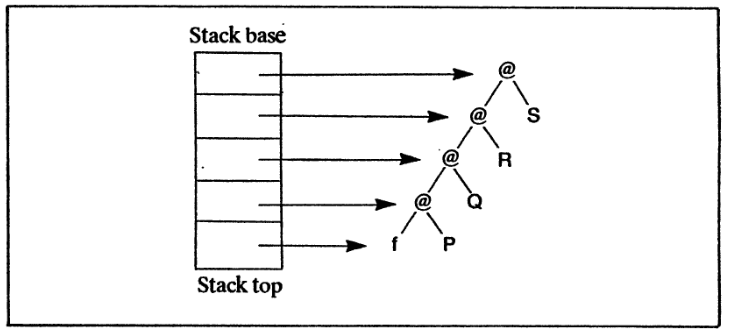
\includegraphics[width=\linewidth]{images/slpj203}
  \caption{Voorbeelden van redex selectie (redex gemarkeerd met '\$')}
  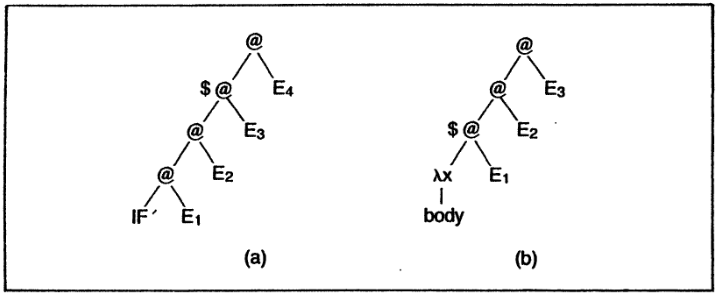
\includegraphics[width=\linewidth]{images/slpj202}
\end{figure}

Wanneer \texttt{f} gevonden is beschouwen we volgende mogelijkheden:
\begin{enumerate}
\item \texttt{f} is een data-object: De expressie is in WHNF dus we zijn klaar.
\item \texttt{f} is een builtin operator of constructor die $k$ argumenten vereist: De expressie is in WHNF als en slechts als $n < k$. In het andere geval is de redex de expressie \texttt{f E1 ... Ek}. De reductie die erop volgt volgt builtin-specifieke regels.
\item \texttt{f} is een $\lambda$-abstractie: Als er een argument beschikbaar is, dan is \texttt{F E1} de redex.
\end{enumerate}
\paragraph{}

\subsection{Graafreductie}
Na het algoritme uit de voorgaande sectie uit te voeren, weten we welke node de redex is, welke de operator, en alle argumenten staan op de spine stack.
Het uitvoeren van een reductie resulteert in een lokale transformatie van de graaf: de redex wordt overschreven door het resultaat van de reductie.
De reductieprocedure wordt bepaald door het type van de operator.
Ten eerste is er het triviale geval dat de operator een \texttt{DATA} cel is: in dit geval moet er niets gebeuren.
\emph{IFPL} maakt verder onderscheid tussen lambda-abstracties en builtin functies. Mijn implementatie beschouwt ook constructors nog als een apart geval.

\subsubsection{Reductie van $\lambda$-abstracties}
In tegenstelling tot strikte talen gaat een luie taal het argument van een functie niet eerst evalueren voordat het argument wordt gesubstitueerd voor de vrije voorvallen van de formele parameter.
Een na{\"i}ve aanpak zou zijn om elk voorval van de formele parameter te vervangen door een kopie van het argument.
Het is makkelijk te zien dat dit tot dubbel werk kan leiden: wanneer de parameter meerdere keren wordt gebruikt in het lichaam van de functie zal mogelijks de evaluatie van de redexes in het argument meerdere keren plaatsvinden.
Verder kan het onge{\"e}valueerde argument zelf redexes bevatten en dus arbitrair groot en complex zijn.
Kopie{\"e}n hiervan maken zou veel geheugen kunnen kosten.
\paragraph{}
De oplossing voor dit probleem is de reden waarom we met grafen en niet met bomen werken: we gaan elk voorval van de parameter vervangen door een \emph{pointer} naar het argument.

\begin{figure}[h]
  \caption{Pointersubstitutie}
  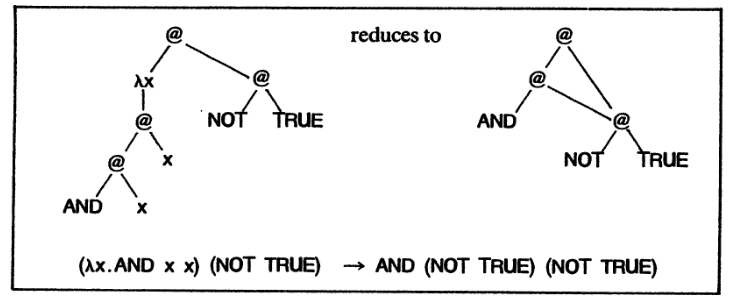
\includegraphics[width=\linewidth]{images/slpj208}
\end{figure}

\paragraph{}
Als een argument nooit wordt gebruikt wordt het nog steeds nooit ge{\"e}valueerd, maar als het resultaat van de evaluatie van een argument minstens 1 keer nodig is, wordt het beschikbaar gemaakt voor alle voorvallen ervan.
\paragraph{}
Het wordt nu ook duidelijk waarom we de wortel van de redex na evaluatie steeds \emph{overschrijven} met het resultaat.
Deze strategie zorgt ervoor dat alle ge{\"i}nteresseerde partijen zonder meerkost een beeld krijgen op het resultaat: de node waar hun pointers naar wijzen wordt aangepast zodat het resultaat steeds onmiddellijk beschikbaar is.

\begin{figure}[h]
  \caption{Overschrijven van de wortel van de redex}
  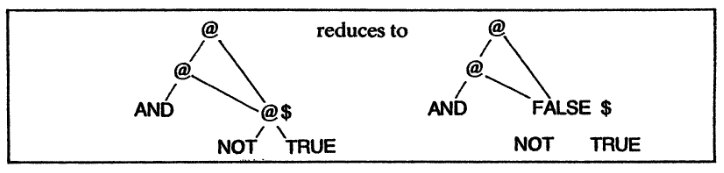
\includegraphics[width=\linewidth]{images/slpj209}
\end{figure}

\paragraph{}
Het is niet onwaarschijnlijk dat een programma meerdere keren dezelfde lambda-abstracties wenst te gebruiken.
Het zal dus niet mogelijk zijn om tijdens het evaluatieproces in het lichaam van de lambda-expressie zelf aanpassingen te maken.
Het is dus nodig om voor elke applicatie van een lambda-expressie een nieuwe kopie te maken van het lichaam, en daarin de nodige substituties te doen.
We voorzien dus een instantiate functie die in 1 pass het lambda lichaam kopieert en waar nodig substituties doet.
\paragraph{}
We hebben nu de essentie van lazy graph reduction beschreven. Het is een strategie die
\begin{enumerate}
\item gebruik maakt van normal-order evaluatie naar WHNF
\item die pointer substitutie gebruikt bij reductie van lambda expressies
\item die de wortel van de gereduceerde expressie steeds overschrijft met het resultaat
\end{enumerate}

\subsubsection{Reductie van builtin functies}
Builtin functies vereisen steeds een vast aantal argumenten voordat reductie kan beginnen (\texttt{+} heeft bijvoorbeeld steeds 2 argumenten nodig), en ze gebruiken vaak ook een afwijkende reductiestrategie voor hun argumenten.

\paragraph{}
Arithmetische of logische functies vereisen bijvoorbeeld steeds dat al hun argumenten volledig gereduceerd zijn (dus geen redexes meer bevatten).
Ze kunnen namelijk enkel opereren op \texttt{DATA} cellen.
Het feit dat volledige reductie moet leiden tot data-objecten zou al verzekerd moeten zijn door de typechecker, dus dit wordt niet gecontroleerd op dit niveau.
Een argument dat eerst volledig gereduceerd moet worden noemen we een \emph{strikt} argument.
De evaluatie van een strikt argument gebeurt nog steeds in \emph{normal order}, maar het reductieproces houdt niet op bij WHNF en gaat door tot normal form.
\paragraph{}
Sommige builtins hebben zeer specifieke eisen wat betreft reductieregels.
Bijvoorbeeld, de \texttt{IF} builtin evalueert eerst zijn eerste argument naar normal form, dan wordt een argument geselecteerd op basis van het resultaat van het eerste argument, wat dan wordt teruggegeven zonder reductie.

\subsubsection{Reductie van constructors}
Mijn implementatie voorziet gestructureerde data met behulp van speciale cellen die een variabele lengte hebben.
Stel dat in de high-level taal een \texttt{LIST} somtype gedefinieerd is, met een \texttt{NIL} en een \texttt{CONS a (LIST a)} constructor.
We hebben dan 1 type met een 0-ary constructor en een binary constructor.
De runtime omgeving moet niet kunnen onderscheiden tussen LIST types en andere types, maar wel tussen NIL en CONS dataobjecten.
De typeinformatie wordt niet meegegeven aan het graafreductiealgoritme.
Het is dus nodig de constructor van een type-onafhankelijke notatie te voorzien die wel informatie over de gebruikte constructor en het benodigd aantal argumenten meedraagt.
Een \texttt{CONSTR} cel bevat dus 2 getallen: een \emph{structured data tag}, een getal dat met een constructor is geassocieerd (bijvoorbeeld 0 stelt een NIL cel voor en 1 een CONS cel), en een \emph{arity}, het nodig aantal argumenten.
\paragraph{}
Ook constructors mogen hun argumenten niet strikt evalueren.
Een gestructureerde datacel moet dus eenvoudigweg verwijzingen naar haar argumenten bijhouden.
Een constructie van de vorm \texttt{CONSTR-t-n a1 ... an} wordt gereduceerd naar een \texttt{DATA} cel die in haar eerste veld de structured data tag $t$ opslaat, en in haar tweede veld een verwijzing naar een array van $n$ \texttt{Cell}-pointers, die elk een verwijzing naar een argument opslaan.
Met een andere ingebouwde functie, \texttt{SELECT}, kan men dan weer de argumenten uit de gestructureerde datacel ophalen.

\end{document}
